\setcounter{chapter}{26}
\chapter{Boundary Conditions for Electric Fields}\label{chap27}

Under static condition, as all charges lie on the outer surface of the conductor, the $\overrightarrow{E}$ and $\overrightarrow{D}$ are zero within the conductor.

\section{Boundary conditions at the conductor-dielectric interface}
\begin{figure}[H]
\centering
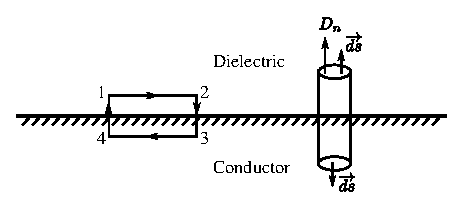
\includegraphics[scale=1.1]{images/fig1.eps}
\caption{Conductor-dielectric interface}\label{chap27-fig1}
\end{figure}

We know that static electric field is a conservative field. 
$$
\text{i.e.,}\qquad \oint \overrightarrow{E} \cdot \overrightarrow{dL} = 0
$$

Consider a closed rectangular path 12341 shown in Fig.~????
\begin{equation}
\oint \overrightarrow{E} \cdot \overrightarrow{dL} = \int_{1}^{2} \overrightarrow{E} \cdot \overrightarrow{dL} + \int_{2}^{3} \overrightarrow{E} \cdot \overrightarrow{dL} + \int_{3}^{4} \overrightarrow{E} \cdot \overrightarrow{dL} + \int_{4}^{5} \overrightarrow{E} \cdot \overrightarrow{dL} = 0\label{chap27-eq1}
\end{equation}

In Eqn.~\eqref{chap27-eq1}, the 3$^{\text{rd}}$ integral is zero because the path 3 to 4 is within the conductor where $\overrightarrow{E}$ is zero. If the path lengths 2 to 3 and 4 to 1 approaches zero (i.e., across boundary), the 2$^{\text{nd}}$ and 4$^{\text{th}}$ integral, in Eqn.~\eqref{chap27-eq2} are zero.
\begin{equation}
\therefore\quad \text{We get } \ \int_{1}^{2} \overrightarrow{E} \cdot \overrightarrow{dL} = \int E_{t}dL = 0\label{chap27-eq2}
\end{equation}

Where $E_{t}$ is the tangential component of $\overrightarrow{E}$ at the surface of the dielectric. 

From Eqn.~\label{chap27-eq2}, we get 
$$
E_{t} = 0\quad \text{\&}\quad D_{t} = 0
$$

Now consider a Gaussian right circular cylinder placed across the boundary as shown in Fig-. From Gauss's law, 
$$
\oint \overrightarrow{D} \cdot \overrightarrow{ds} = Q_{\text{enclosed}}.
$$
\begin{equation}
\int\limits_{\text{top}} \overrightarrow{D} \cdot \overrightarrow{ds} + \int\limits_{\text{bottom}} \overrightarrow{D} \cdot \overrightarrow{ds} + \int\limits_{\text{side}} \overrightarrow{D} \cdot \overrightarrow{ds} = \int_{s} P_{s}ds\label{chap27-eq3}
\end{equation}

In Eqn.~\eqref{chap27-eq3}, the 2$^{\text{nd}}$ integral is zero because the bottom of the cylinder is within the conductor where $\overrightarrow{D}$ and $\overrightarrow{E}$ are zero. The 3$^{\text{rd}}$ integral is zero because $D_{t} = 0$. 
\begin{align*}
\therefore \ & \oint\limits_{\text{top}} \overrightarrow{D} \cdot \overrightarrow{ds} = \int\limits_{\text{top}} D_{n}ds = \int_{s} \rho_{s}ds\\
\therefore \ & D_{n} = \rho_{s} ~\&~ E_{n} = \dfrac{\rho_{s}}{\epsilon}
\end{align*}

\section{Boundary conditions at the dielectric-dielectric interface}\label{chap27-sec2}
\begin{figure}[H]
\centering
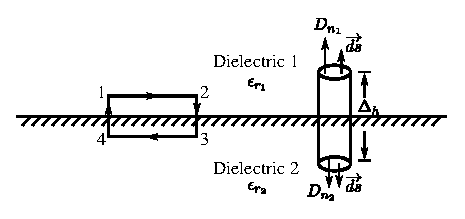
\includegraphics[scale=1.1]{images/fig2.eps}
\caption{Dielectric-dielectric interface}\label{chap27-fig2}
\end{figure}


Consider a dielectric - dielectric interface as shown in Fig.~\ref{chap27-fig2}

Applying Eqn.~\eqref{chap27-eq4} to the closed path 12341,
\begin{equation}
\int_{1}^{2} \overrightarrow{E} \cdot \overrightarrow{dL} + \int\limits_{2}^{3} \overrightarrow{E} \cdot \overrightarrow{dL} + \int\limits_{3}^{4} \overrightarrow{E} \cdot \overrightarrow{dL} + \int\limits_{4}^{1} \overrightarrow{E} \cdot \overrightarrow{dL} = 0\label{chap27-eq4}
\end{equation}

In Eqn.~\eqref{chap27-eq4}, if the path lengths 2 to 3 and 4 to 1 approaches zero (i.e.., across boundary), the 2$^{\text{nd}}$ and 4$^{\text{th}}$ integrals are zero. 
\begin{align*}
\therefore\quad  &\int\limits_{1}^{2} \overrightarrow{E} \cdot \overrightarrow{dL} + \int\limits_{3}^{4} \overrightarrow{E} \cdot \overrightarrow{dL} = 0\\
 & \int E_{t_{1}}dL - \int E_{t_{2}}dL  = 0\\
 & \int \left(E_{t_{1}} - E_{t_{2}}\right)dL  = 0\\
 & E_{t_{1}} - E_{t_{2}} = 0
\end{align*} 
$$
\therefore\quad E_{t_{1}} = E_{t_{2}} \quad\text{\&}\quad \dfrac{D_{t_{1}}}{\varepsilon_{r_{1}}} = \dfrac{Dt_{2}}{\varepsilon_{r_{2}}}
$$
Therefore across dielectric-dielectric interface 
tangential component of $\overrightarrow{E}$ is continuous cylindrical. 

Applying Eqn~.\eqref{???}, to the Gaussian surface, 
\begin{equation}
\int\limits_{\text{top}} \overrightarrow{D} \cdot \overrightarrow{ds} + \int\limits_{\text{bottom}} \overrightarrow{D} \cdot \overrightarrow{ds} + \int\limits_{\text{side}} \overrightarrow{D} \cdot \overrightarrow{ds} = \int\limits_{s} P_{s}ds\label{chap27-eq27.5}
\end{equation}

In Eqn.~\eqref{chap27-eq27.5}, as $\Delta h$ approaches zero (i.e., across boundary) the 3$^{\text{rd}}$ integral in Eqn.~???? is zero. The RHS of Eqn.~???? is zero because is dielectric $\rho_{s} = 0$.
\begin{align*}
& \int\limits_{\text{top}} \overrightarrow{D} \cdot \overrightarrow{ds} + \int\limits_{\text{bottom}} \overrightarrow{D} \cdot \overrightarrow{ds} = 0\\
& \int Dn_{1}ds - \int Dn_{2}ds  = 0\\
& \int (D_{n_{1}} - D_{n_{2}})ds = 0\\
& D_{n_{1}} - D_{n_{2}}  = 0
\end{align*}
$$
\therefore\quad  D_{n_{1}} = D_{n_{2}}  \quad\text{\&}\quad \varepsilon_{r_{1}}E_{n_{1}} = \varepsilon_{r_{2}}E_{n_{2}}. 
$$
Therefore across dielectric-dielectric interface normal component of $\overrightarrow{D}$ is continuous. 

\begin{problem}
Given that $\overrightarrow{E_{1}} = 2\overrightarrow{a_{x}} - 3\overrightarrow{a_{y}} + 5\overrightarrow{a_{z}}$ across dielectric-dielectric interface shown in Fig.~\ref{chap27-fig3}. Find $\overrightarrow{E_{2}}, \overrightarrow{D_{1}}, \overrightarrow{D_{2}}$ and the angles $\theta_{1}$ and $\theta_{2}$. 
\begin{figure}[H]
\centering
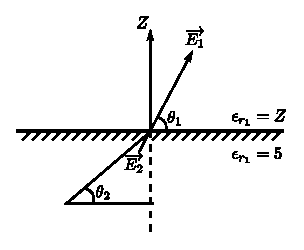
\includegraphics[scale=1.1]{images/fig3.eps}\label{chap27-fig3}
\end{figure}
\end{problem}

\begin{solution}
$\overrightarrow{a_{x}}$ and $\overrightarrow{a_{y}}$ are tangential \& $\overrightarrow{a_{2}}$ is normal to the interface

Given : $\overrightarrow{E_{1}} = 2\overrightarrow{a_{x}} - 3\overrightarrow{a_{y}} + 5\overrightarrow{a_{z}}$
$$
\therefore\quad \overrightarrow{D_{1}} = \varepsilon_{0}\varepsilon_{r_{1}} = 4\varepsilon_{0}\overrightarrow{a_{x}} - 6\varepsilon_{0}\overrightarrow{a_{y}} + 10\varepsilon_{0}\overrightarrow{a_{z}}
$$

From Eqns. ????? \& ?????
\begin{align*}
\overrightarrow{E_{2}} & = 2\overrightarrow{a_{x}} - 3\overrightarrow{a_{y}} + \left(\dfrac{2}{5}\right) 5\overrightarrow{a_{z}}\\
\therefore\quad \overrightarrow{E_{2}} & = 2\overrightarrow{a_{x}} - 3\overrightarrow{a_{y}} + 2\overrightarrow{a_{z}}\\
\overrightarrow{D_{2}} & = \left(\dfrac{5}{2}\right) + \varepsilon_{0}\overrightarrow{a_{x}} - \left(\dfrac{5}{2}\right) 6\varepsilon_{0}\overrightarrow{a_{y}} + 10\varepsilon_{0}\overrightarrow{a_{z}}\\
\therefore\quad \overrightarrow{D_{2}} & = 10\varepsilon_{0}\overrightarrow{a_{x}} - 15\varepsilon_{0}\overrightarrow{a_{y}} + 10\varepsilon_{0}\overrightarrow{a_{z}}
\end{align*}

From Fig.~????
\begin{align*}
E_{z_{1}} & = \overrightarrow{E_{1}} \cdot \overrightarrow{a_{z}} = E_{1} \cos (90 - \theta_{1})\\
&\quad 5 = \sqrt{2^{2} + 3^{2} + 5^{2}} \sin \theta_{1}\\
&\quad \theta_{1} = 54.2^{\circ}\\[0.3cm]
E_{z_{2}} & = \overrightarrow{E_{2}} \cdot \overrightarrow{a_{z}} = E_{2} \cos (90 - \theta_{2})\\
&\quad 2 = \sqrt{2^{2} + 3^{2} + 2^{2}} \sin \theta_{2}\\
&\quad \theta_{2} = 29.0^{\circ}
\end{align*}
\end{solution}

\begin{problem}
At the boundary between given ($\varepsilon_{r} = 4$) and air, the lines of electric field makes an angle of $40^{\circ}$ with normal to the boundary. If the electric flux density in air is $0.25 \mu$ c/m$^{2}$, determine the orientation and magnitude of electric flux density in glass. 

\hfill [VTU : Jan 2005, Aug 2001]
\end{problem}

\begin{solution}
~

\begin{figure}[H]
\centering
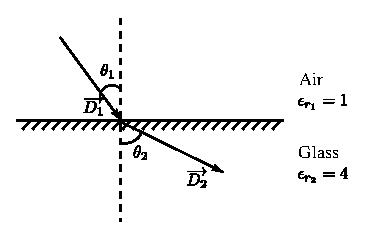
\includegraphics[scale=1.1]{images/fig4.eps}\label{chap27-fig4}
\end{figure}

For dielectric-dielectric interface,
\begin{align}
D_{t_{1}} & = \dfrac{\varepsilon_{r_{1}}}{\varepsilon_{r_{2}}} \cdot D_{t_{2}}\notag\\
D_{1} \sin \theta_{1} & = \dfrac{1}{4} D_{2} \cdot \sin \theta_{2}\label{??}\\
D_{n_{1}} & = D_{n_{2}}\notag\\
D_{1} \cos \theta_{1} & = D_{2} \cos \theta_{2}\label{??}\\
\therefore\quad \tan \theta_{1} & = \dfrac{1}{4} \tan \theta_{2}\notag\\
\tan 40 & = \dfrac{1}{4} \tan \theta_{2}\notag\\
\therefore\quad \theta_{2} & = 73.41^{\circ}\notag
\end{align}

Given that $D_{1} = 0.25\mu$ c/m$^{2}$,

From: Eqn.~???, 
\begin{gather*}
0.25\times 10^{-16} \times \cos 40 = D_{2} \cos 73.41\\
\therefore\quad D_{2} = 0.67\mu \text{c/m}^{2}
\end{gather*}
\end{solution}

\begin{problem}
An electric field strength 1.2 V/m is entering a dielectric medium of $\epsilon_{r} = 4$ from air. The orientation of the electric field in air is $65^{\circ}$ w.r.t the boundary. Determine the orientation and the strength of the electric field in the dielectric medium. 
\end{problem}

\begin{solution}
~

\begin{figure}[H]
\centering
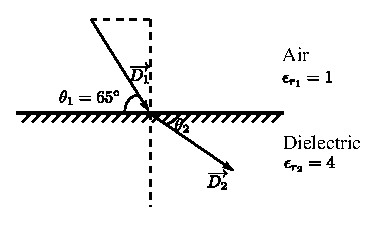
\includegraphics[scale=1.1]{images/fig5.eps}\label{chap27-fig5}
\end{figure}

Across dielectric-dielectric boundary, 
\begin{align}
E_{t_{1}} & = E_{t_{2}}\notag\\
E_{1} \cos \theta_{1} & = E_{2} \cos \theta_{2}\label{}\\
\varepsilon_{r_{1}}E_{n_{1}} & = \varepsilon_{r_{2}}E_{n_{2}}\notag\\
E_{n_{1}} & = \dfrac{\varepsilon_{r_{2}}}{\varepsilon_{r_{1}}} E_{n_{2}}\notag\\
E_{1} \sin \theta_{1} & = \dfrac{\varepsilon_{r_{2}}}{\varepsilon_{1}} E_{2} \sin \theta_{2}\label{???}\\
\therefore\quad \tan \theta_{1} & = \dfrac{\varepsilon_{r_{2}}}{\varepsilon_{1}} \tan \theta_{2}\notag\\
\tan 65 & = \dfrac{4}{1} \tan \theta_{2}\notag\\
\therefore\quad \theta_{2} & = 28.2^{\circ}\notag
\end{align}

Given that $E_{1} = 1.2 Vm^{-1}$

From 
\begin{align*}
1.2\cos 65 & = E_{2} \cos 28.2\\
\therefore\quad E_{2} & = 0.575 V/m
\end{align*}
\end{solution}


\begin{problem}
In region $1 ; (z < 0m)$ (free space) where $D_{1} = 5\overrightarrow{a_{y}} + 7\overrightarrow{a_{z}} \text{c/m}^{2}$; region $2 ; (0 < z < 1m)$ has $\epsilon_{r_{2}} = 2.5$ and region $3 ; (z > 1m)$ has $\epsilon_{r_{3}} = 3.0$

Find $E_{1}, D_{2}, E_{2}, D_{3}, E_{3}$ and $\theta_{3}$
\end{problem}

\begin{solution}
~

\begin{figure}[H]
\centering
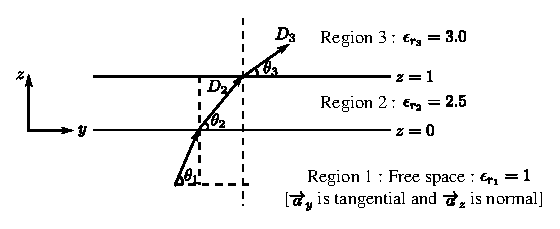
\includegraphics[scale=1.1]{images/fig6.eps}\label{chap27-fig6}
\end{figure}

Given:
\begin{align*}
\overrightarrow{D_{1}} & = 5\overrightarrow{a_{y}} + 7\overrightarrow{a_{z}}\\
\overrightarrow{E_{1}} & = \dfrac{\overrightarrow{D_{1}}}{\varepsilon_{0}} = \dfrac{1}{\varepsilon_{0}} [5\overrightarrow{a_{y}} + 7\overrightarrow{a_{z}}]\\
D_{2} & = \left(\dfrac{2.5}{1}\right) 5\overrightarrow{a_{y}} + 7\overrightarrow{a_{z}} = 12.5\overrightarrow{a_{y}} + 7\overrightarrow{a_{z}}\\
\overrightarrow{E_{2}} & = \dfrac{1}{\varepsilon_{0}\varepsilon_{r_{2}}} \overrightarrow{D_{2}} = \dfrac{1}{\varepsilon_{0}} \left[5\overrightarrow{a_{y}} + \dfrac{7}{2.5} \overrightarrow{a_{z}}\right]\\
\overrightarrow{D_{3}} & = \left(\dfrac{3}{2.5}\right) 12.5\overrightarrow{a_{y}} + 7\overrightarrow{a_{z}} = 15\overrightarrow{a_{y}} + 7\overrightarrow{a_{z}}\\
\overrightarrow{E_{3}} & = \dfrac{1}{\varepsilon_{0}\varepsilon_{r_{3}}} \overrightarrow{D_{3}} = \dfrac{1}{\varepsilon_{0}} \left[5\overrightarrow{a_{y}} + \dfrac{7}{3} \overrightarrow{a_{z}}\right]
\end{align*}

From Fig.~: 
\begin{align*}
D_{z_{3}} & = \overrightarrow{D_{3}} \cdot \overrightarrow{a_{z}} = D_{3} \cos (90 - \theta_{3})\\
7 & = \sqrt{15^{2} + 7^{2}} \sin \theta_{3}\\
\therefore \theta_{3} & = 25.02^{\circ}
\end{align*}
\end{solution}

\label{27end}

